\begin{figure}[ht!]
  \centering
  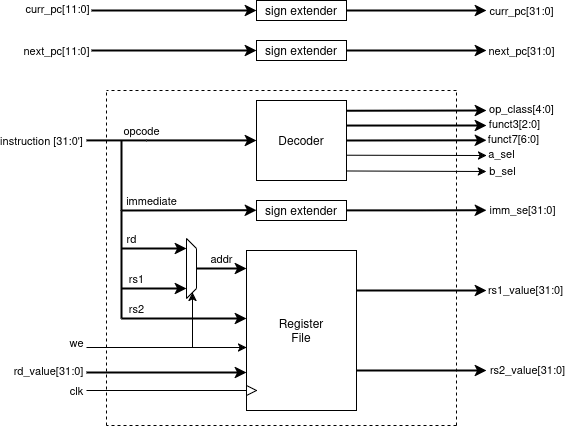
\includegraphics[scale=0.4]{ID_BD.png}
  \caption{A block diagram for the instruction decoding stage}
  \label{fig:ID_BD}
\end{figure}

After the instruction is returned from the fetching stage, it must be decoded in order to select the right action to be performed in the next step of the datapath. RISC-V ISA provides instructions for registers to operate with other registers, constants, Data Memory or the PC itself and there is the necessity to distinguish what parts of the instruction make up the operands of the execution and where the resulting information has to be stored.
This action is done by the Instruction Decode, which selects what to use as operands through the multiplexers located at the upcoming stage, while also recognizing and subsequently giving more information about the instruction to the ALU.
There are four core instruction formats that encode said informations:
\begin{itemize}
\item \textbf{R-type}: Register to register instructions. These instructions are expected to use two registers as sorce for data to be elaborated and then store the result of the operation in a destination register.
\begin{minted}{gas}
                  add rd, rs1, rs2       ; rd = rs1 + rs2
\end{minted}
This instruction has to select the two source registers as operands in the ALU, hence two boolean outputs \emph{a\_sel} and \emph{b\_sel} will be pulled high to indicate to the ALU that the registers pointed by the values of rs1 (bits 19 down to 15 of the 32 bits instruction) and rs2 (bits 24 down to 20).
\item \textbf{I-type}: These ones have a constant value, i.e. an immediate, encapsulated in the code, that becomes be part of the operation. Some examples are:
\begin{minted}{gas}
                  addi rd, rs1, imm         ; rd = rs1 + imm
                  lw rd, imm(rs1)           ; rd = Mem[rs1 + imm]
\end{minted}
The value stored in rs1 is encapsulated in bits 19 down to 15 and the immediate value from bit 31 to 20. \emph{a\_sel} has to be set high while \emph{b\_sel} is set to low.
\item \textbf{S-type}: For store operations, where the content of the register rs2 is stored inside the memory address in the data memory pointed by rs2, possibly summed to an immediate value (little endian encoded, bits 31 to 25 for the 7 most significant bits and bits 11 to 7 for the least significant ones). 
\begin{minted}{gas}
                  sw rs2, imm(rs1)          ; Mem[rs1 + imm] = rs2
\end{minted}
In this case \emph{a\_sel} is set to high while \emph{b\_sel} stays low in order for the ALU to sum rs1 and the immediate value.
\item \textbf{U-type}: Loading immediates inside a register, like for example LUI (Load Upper Immediate, also known as the pseudo-instruction li). In this case \emph{b\_sel} is set to be low while \emph{a\_sel} can be either high or low, as the ALU can be programmed to ignore the first operand if necessary.
\begin{minted}{gas}
                  lui rd, imm               ; rd = imm
\end{minted}
\end{itemize}
\subsection{Instruction formats}
\begin{figure}[h!]
  \centering
  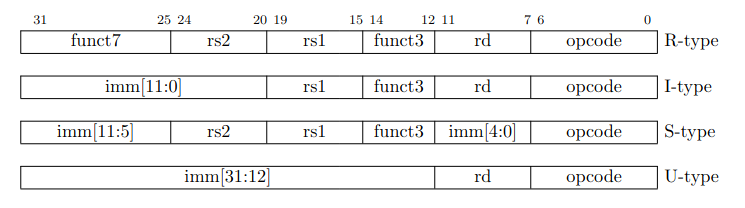
\includegraphics[scale=0.6]{base_isa.png}
  \caption{Base instruction format \cite{waterman2016riscv}}
  \label{fig:base_form}
\end{figure}
These instructions share the same positions for the operands and the destination registers, which simplifies the structure of the code (Figure \ref{fig:base_form}).
Instructions that operate with the PC and conditional instructions such as branches share similar structure with respectively U-type and S-type instructions, in the ISA they are defined as:
\begin{itemize}
  \item \textbf{B-type} or SB-type: Just as in store operations, the rs1 and rs2 addresses are coded in the same position, with the difference that the immediate value has its bits coded in different positions (imm[12] on bit 31, imm[11] on bit 7, imm[10:5] from bit 30 to 25, imm[4:1] from bit 11 to 8). For this type of operation there is no need to change \emph{a\_sel} and \emph{b\_sel}, since, as it will be shown later, the logic unit just operates between registers.
  \item \textbf{J-type} or UJ-type: Jump operations sums an immediate to the PC and stores the next instruction's PC value. These are coded just as unsigned operations, with the difference being the immediate's bits having different positions (imm[20] on position 31, imm[19:12] from position 19 to 12, imm[11] on bit 20 and imm[10:1] from position 30 to 21).
\end{itemize}
With these definitions, the base ISA extends to this:
\begin{figure}[ht]
  \centering
  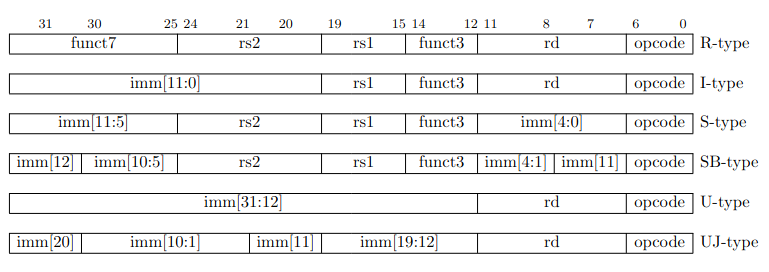
\includegraphics[scale=0.58]{base_isa_2.png}
  \caption{Full 32-bit instruction format \cite{waterman2016riscv}}
  \label{fig:full_form}
\end{figure}
Knowing that the next block can be programmed to use certain parts of the instruction in a certain way, the VHDL code for the ID architecture can be simplified by giving out all the sections of the instruction and letting the Instruction Execute select what specific parts of it are needed.

\subsection{Decoding}
\subsubsection{Reading opcodes for operand selection}
The encoding type of an instruction is not sufficient to detect what operation is actually performed. For example, \emph{LW} and \emph{ADDI} are both I-type instructions but the latter has its result written somewhere in the Register File instead of the Data Memory.
For this reason it is necessary to assess some information segments inside the instruction itself. By looking at Figure \ref{fig:full_form} it is noticeable that there are at most three elements that are descriptive of the content of the instruction and its behavior:
\begin{itemize}
  \item \textbf{opcode}: Unique and present in every instruction, composed by the first 7 bits (starting from the LSB, considering a Little Endian encoding).
  \item \textbf{funct3}: Present in all instructions but U and J -types, made by bit 12 up to 14, necessary for the ALU to select the arithmetic or logic operation to be executed.
  \item \textbf{funct7}: Only for R-type instructions, in the RV32I ISA only one of the seven bits is used.
\end{itemize}
It's obvious that \emph{funct3} and \emph{funct7} do not give information about the identity of the instruction, it is the \emph{opcode} that differentiates the operation and therefore the one that has to be taken into account. The Instruction Set manual [described by Waterman et al. (2016) \cite{waterman2016riscv} page 53 Table 9.1] gives the general opcode map that can help to discriminate instructions: 

\begin{figure}[h!]
  \centering
  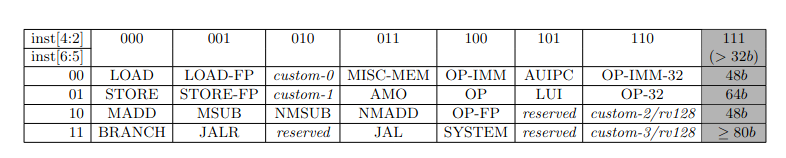
\includegraphics[scale=0.55]{opcodes.png}
  \caption{RISC-V base opcode map, RISC-V user-level ISA version 2.1 \cite{waterman2016riscv}} 
  \label{fig:opcode_map}
\end{figure}

The opcode map gives the idea that a decoder can be described with a nested case statement, with an external case structure driven by the last two bits of the opcode, from which is possible to extrapolate what are the operands to be passed to the ALU or Logic Unit, being it the PC, two registers or an immediate and a register.  

\subsubsection{Instruction classification}
The last and most delicate problem that arises when decoding instructions is that they operate in different ways even if they share the same encoding type, for example, ADDI (I-type) will write the result of the arithmetic operation in a destination register, while LW (I-type) will have as destination register a memory location pointed by the result of another arithmetic operation. Also, the interaction with the PC can widely differ based off the circumstances, hence there is the additional requirement to define in advance a classification method so that the Write Back stage can select what can has to be passed to the Register File and select the next value for the Program Counter. There are three possible cases in which the Write Back accesses the register file: Jumps (since they write back the return address), Loads and arithmetic/logic operations; In addition, the PC can have a new value loaded if, during a branch intruction, the Logic Unit returns a logic high, or during a jump instruction. Otherwise, PC+4 is always returned as next value.\\
The solution could be encoding these informations for the next stages as a 6 bit vector, with a one-hot encoding for Arithmetic-Logic Operations, Jump, Load and Store,since store operations can be added as an additional bit that can be used as a write-enable for the Data Memory.\\
Some instructions though cannot follow this pattern, for example, \emph{Load Upper Immediate} (U-type) takes the 32 bit immediate, with the bits 31 downto 12 being the ones the user can manipulate and the remaining 11 downto 0 being filled with zeros, and loads it to a destination register; No operation other than returning a constant is being made yet it is not a load operation nor an arithmetic or logic operation. The same thing happens for AUIPC with the difference being that the resulting immediate is alse added to the PC.\\
To solve this problem the 6 vector could instead not be one-hot encoded and possibly include these instructions that, at first glance, could actually seem like a combination of multiple types, for example, if operations are visualized as "000010" and load operations as "000100", then LUI can be encoded as "000110". This could actually be a fine solution, opcode map Figure \ref{fig:opcode_map} might tell otherwise if the purpose of this project was its expansion to include floating-point operations and multiplications, yet they could actually be encoded as simple operations, letting the ALU manage them in function of \emph{funct7} and \emph{funct3}, while system instruction can be easily encoded as instruction class "000000" or similarly as other instruction if necessary.

\subsection{Register File}
The Register File (Source Code \ref{code:reg_file}) is the last block needed to complete the stage. In these architectures is made by 32 register, each one with a length of 32 bits which greatly simplifies its imlementation in VHDL by declaring it as an array of logic vectors.
The register as VHDL entity can be defined as a three port RAM that allows read and write operations in the same clock cycle without the need of a correct timing, as it would happen in double port RAMs; Write operations will be performed at the rising edge of the clock if a write-enabling input is set to logic high, while read operation can be asynchronous to the clock. In addition, every write operation to the x0 register will be ignored as by RISC-V specification.

\subsection{Final concept for the ID and simulation}
With the current initialization files for the IM, only a small amount of instructions are going to be tested, for this reason the new file should contain each existing tipology, possibly testing the ones that use \emph{funct7} while also implementing jumps and branches, possibly with a loop so that the next stages can be easily tested for inconsistencies or error that may stop the code from running.The new initialization could become:

\begin{minted}{text}
memory_initialization_radix = 16;
memory_initialization_vector =
000100b7,   --> lui x1, 0x10
00408113,   --> addi x2, x1, 4
002081b3,   --> add x3, x1, x2
0030a223,   --> sw x3, 4(x1)
0040a203,   --> lw x4, 4(x1)
404182b3,   --> sub x5, x3, x4
0000006f,   --> jal x0, 0 
fe108ee3;   --> beq x1, x1, -8
\end{minted}

The finalized concept of the Instruction decode, which follows the block diagram at Figure \ref{fig:ID_BD}, introduces the Register File and a specialized block for decoding, taking as inputs all the IF's outputs (including {pc\_out} and {next\_pc} for sign extension).
The most complex part of this stage, the decoder, is implemented as specified earlier, with two nested case statements, with the outer statement using the two most significant bits of the opcode. A snippet is provided at Source Code \ref{code:ID_decoder}.
By using the same testbench as for the IF and istantiating the ID (Notes Code \ref{code:ID_TB}), by routing the selected instruction and the PC's values, the code is expected to fetch the instruction 0x000100b7, decode it and classify it as an operation with an immediate as second operand, hence with \emph{a{\_}sel}=1, \emph{b{\_}sel}=0 and \emph{op{\_}class}=000110, in fact:

\begin{figure}[h!]
  \centering
  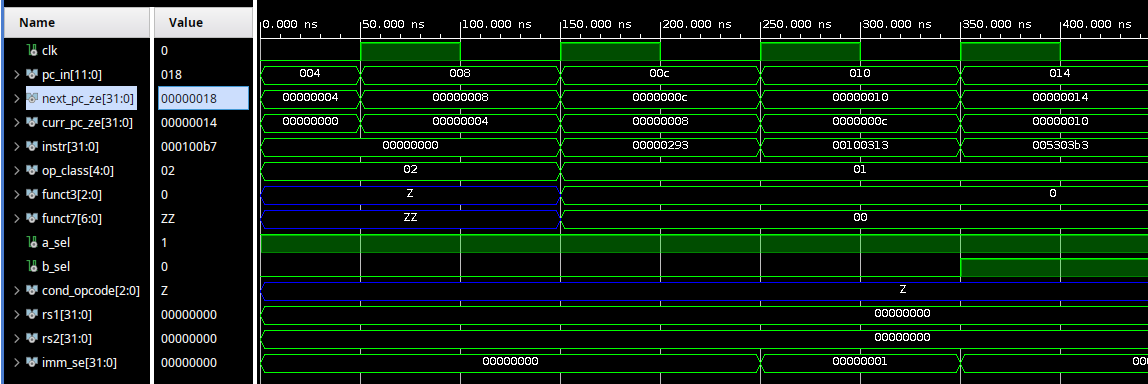
\includegraphics[scale=0.37]{ID_sim.png}
\end{figure}

One particular oservation that could be made is that the Decoder, at any point where the IM returns an empty instruction, i.e. with its hexadecimal value at 0, is going to report it as a LOAD instruction (\emph{op{\_}class} = "000100") if the first two bits of the instruction are not read. This id due to the fact that if the first two bits (that should always be "11" in RV32) are ignored, the decoder will select the firt case as true, thus performing a load operation. For this reason, even if they can be ignored, the caase statement will take them into account to avoid problems with empty IM addresses.